
\subsection{BP 7:
 Monai valley beach (Laboratory)}

{\bf Documentation:}  PMEL-135, pp 6 \& 45-46.

\subsubsection{Problems encountered}

\begin{itemize}
\item The input data only goes out to 20 seconds.

\item The first waves are modeled well but later waves are not seen in the
computation.  This is perhaps related to first point.  

\item Data is not provided for run-up in the valley.
\end{itemize}

\subsubsection{What we did}

\begin{itemize}
\item Used $g=9.81$ and no friction.
\item Used given initial wave to specify a boundary condition at the left
boundary up to time 20.
\item After time 20, switched to non-reflecting at left boundary, so
reflected waves exit.  
(Wave tank was much longer than computational domain specified.)
\item Solved on $423\times 243$ grid (same as bathymetry)
\item Solved on $160\times 100$ grid (not aligned with bathymetry)
\end{itemize} 

\subsubsection{Gauge comparisons}

See \Fig{bp7gauges}.

\begin{figure}[ht]
\hfil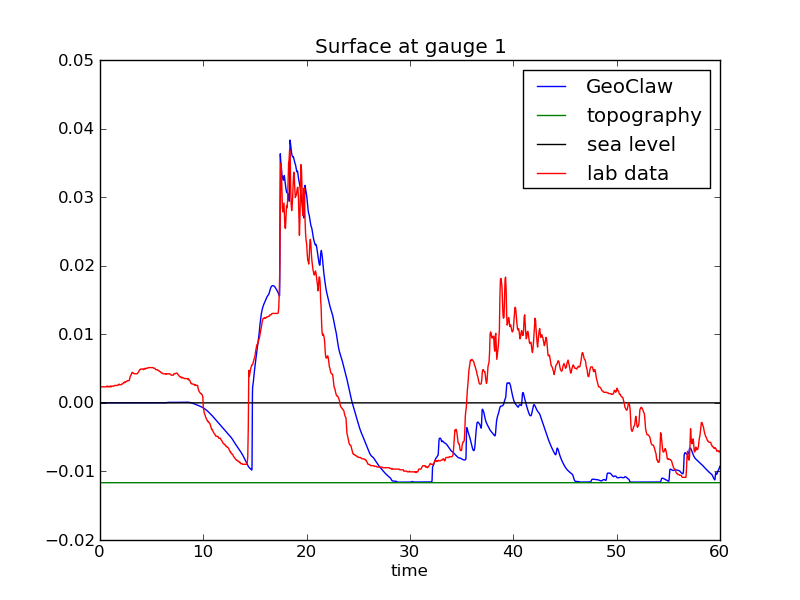
\includegraphics[width=2.8in]{bp7/figs423/gauge0001fig300.png}\hfil
\hfil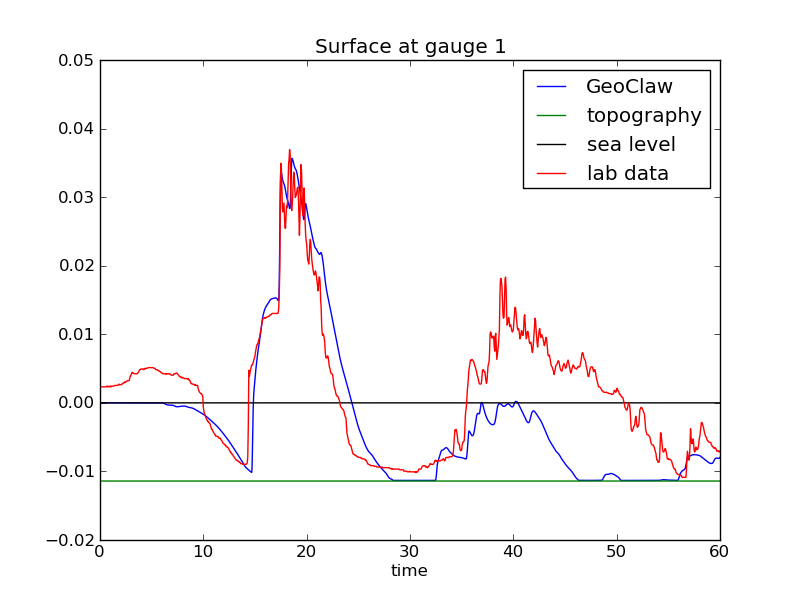
\includegraphics[width=2.8in]{bp7/figs160/gauge0001fig300.png}\hfil
\vskip 5pt
\hfil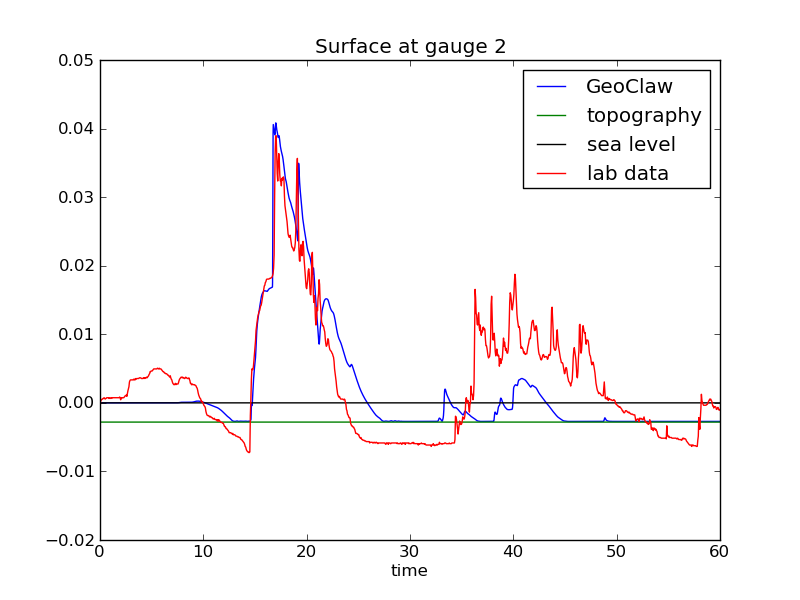
\includegraphics[width=2.8in]{bp7/figs423/gauge0002fig300.png}\hfil
\hfil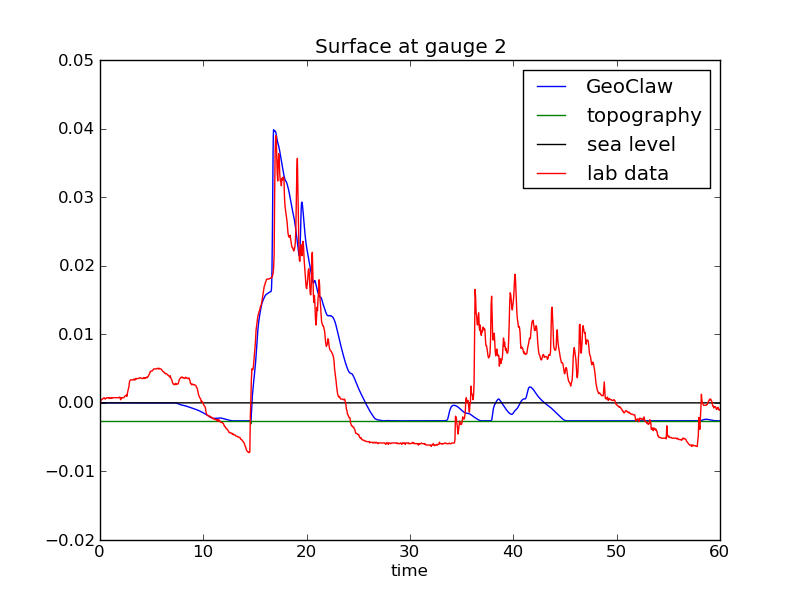
\includegraphics[width=2.8in]{bp7/figs160/gauge0002fig300.png}\hfil
\vskip 5pt
\hfil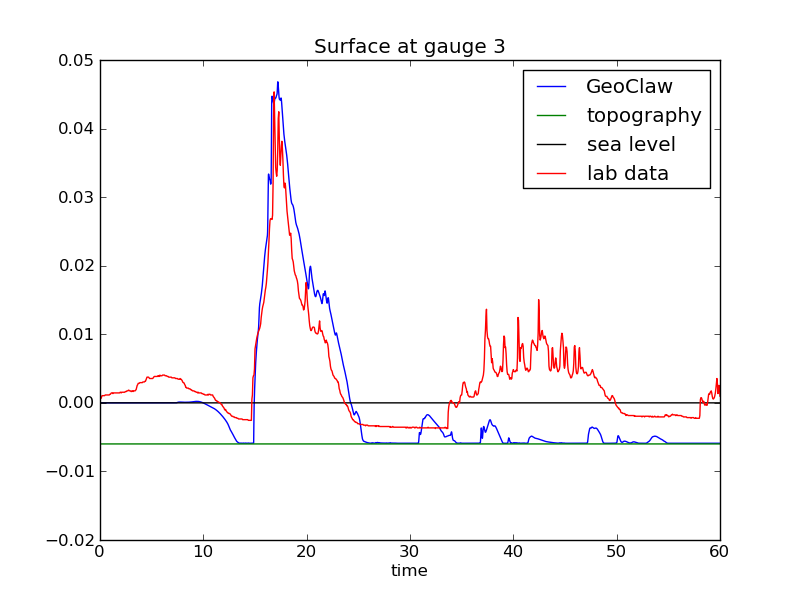
\includegraphics[width=2.8in]{bp7/figs423/gauge0003fig300.png}\hfil
\hfil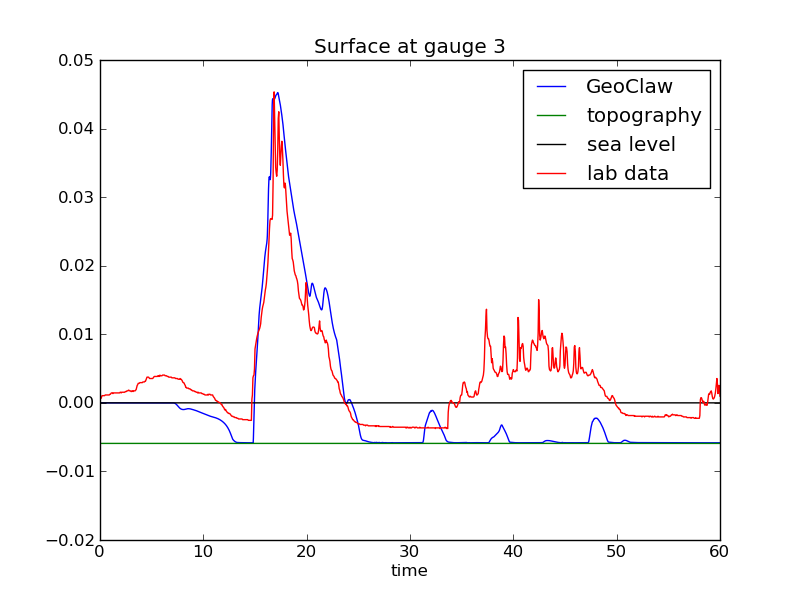
\includegraphics[width=2.8in]{bp7/figs160/gauge0003fig300.png}\hfil
\caption{\label{fig:bp7gauges} 
Left column: on $423\times 243$ grid (same as given bathymetry).
Right column: $160\times 100$ grid (coarser and not aligned with
bathymetry).
  }
\end{figure}

\subsection{Lessons learned}

(Make any relevant comments or observation regarding the benchmark itself,
the available data provided, the relevance of the benchmark to tsunami
science in general and to validating your specific model in particular. 
Report problems and make recommendations regarding improving the benchmark
or its data, as appropriate.)

